% Chat Scratchy — Product Presentation (English deck; Chinese UI screenshots)
% Compile with: xelatex deck.tex   (needs Noto Sans)
\documentclass[aspectratio=169,11pt]{beamer}

\usepackage{fontspec}
\usepackage{graphicx}
\usepackage{tikz}
\usetikzlibrary{shadows.blur,arrows.meta,positioning,calc,fit,backgrounds}

% Let beamer defer all font choices to fontspec.
\usefonttheme{professionalfonts}
\setmainfont{Noto Sans}
\setsansfont{Noto Sans}
\renewcommand{\familydefault}{\sfdefault}
\newcommand{\headingfont}{\bfseries}

% ── Palette (matches the app's pink→purple identity) ──────────────────────
\definecolor{scPurple}{HTML}{7C3AED}
\definecolor{scPink}{HTML}{EC4899}
\definecolor{scInk}{HTML}{1F2937}
\definecolor{scGray}{HTML}{6B7280}
\definecolor{scBg}{HTML}{F3EEF8}
\definecolor{scGreen}{HTML}{22C55E}
\definecolor{scBlue}{HTML}{3B82F6}

% ── Theme ─────────────────────────────────────────────────────────────────
\usetheme{default}
\setbeamertemplate{navigation symbols}{}
\setbeamercolor{frametitle}{fg=scInk}
\setbeamercolor{normal text}{fg=scInk}
\setbeamercolor{itemize item}{fg=scPink}
\setbeamercolor{itemize subitem}{fg=scPurple}
\setbeamerfont{frametitle}{series=\bfseries,size=\LARGE}
\setbeamertemplate{itemize item}{\textbullet}
\setbeamertemplate{itemize subitem}{\textendash}

\setbeamertemplate{frametitle}{%
  \vspace*{0.55em}%
  \begin{beamercolorbox}[wd=\paperwidth,leftskip=0.9cm,rightskip=0.9cm]{frametitle}%
    {\color{scPink}\rule{4pt}{0.95em}}\hspace{0.4em}{\headingfont\insertframetitle}%
  \end{beamercolorbox}%
}
\setbeamertemplate{footline}{%
  \hfill{\color{scGray}\scriptsize\insertframenumber\,/\,\inserttotalframenumber}\hspace{0.7cm}\vspace{0.3cm}%
}

% ── Helpers ────────────────────────────────────────────────────────────────
\newcommand{\shot}[2][0.84\paperheight]{%
  \begin{center}%
  \begin{tikzpicture}%
    \node[inner sep=0pt,draw=scGray!30,line width=0.6pt,rounded corners=3pt,
          blur shadow={shadow blur steps=8,shadow xshift=0pt,shadow yshift=-1pt,shadow opacity=25}]
      {\includegraphics[height=#1,keepaspectratio]{#2}};%
  \end{tikzpicture}%
  \end{center}%
}
% Caption on a translucent backdrop so it stays readable over a screenshot.
\newcommand{\shotcaption}[1]{%
  \begin{tikzpicture}[remember picture,overlay]
    \node[anchor=south,rounded corners=5pt,
          fill=white,fill opacity=0.88,text opacity=1,
          draw=scGray!25,line width=0.4pt,
          text=scInk,font=\scriptsize,text width=0.84\paperwidth,align=center,inner sep=6pt]
      at ([yshift=0.32cm]current page.south) {#1};
  \end{tikzpicture}}
\newcommand{\bgband}{%
  \begin{tikzpicture}[remember picture,overlay]
    \fill[scPurple] (current page.south west) rectangle (current page.north east);
    \fill[scPink,opacity=0.55] (current page.south west) -- (current page.south east)
      -- ([yshift=2.2cm]current page.east) -- ([yshift=-1.2cm]current page.west) -- cycle;
  \end{tikzpicture}}
% numbered badge for the pillar cards
\newcommand{\badge}[2]{\tikz[baseline=-0.6ex]\node[circle,fill=white,text=#1,
  font=\bfseries\large,inner sep=2pt,minimum size=1.0em]{#2};}

\title{Chat Scratchy}
\date{}

\begin{document}

% ─────────────────────────── TITLE ───────────────────────────
{\setbeamertemplate{footline}{}
\begin{frame}[plain]
  \bgband
  \begin{tikzpicture}[remember picture,overlay]
    \node[anchor=west,text=white] at ([xshift=1.0cm,yshift=1.5cm]current page.west) {%
      \begin{minipage}{0.84\paperwidth}
        {\headingfont\fontsize{42}{48}\selectfont Chat Scratchy}\\[0.35em]
        {\fontsize{17}{22}\selectfont An AI coding tutor \;+\; a live classroom dashboard}\\[1.2em]
        {\color{white!88}\fontsize{12}{16}\selectfont Kids learn to code with blocks while an AI tutor guides them ---\\
         and teachers watch the whole class at a glance.}
      \end{minipage}};
    \node[anchor=south west,text=white!80,font=\scriptsize] at ([xshift=1.05cm,yshift=0.8cm]current page.south west)
      {React 19 \, $\cdot$ \, Google Blockly \, $\cdot$ \, Express \, $\cdot$ \, PostgreSQL \, $\cdot$ \, SSE \, $\cdot$ \, LLM tutor};
  \end{tikzpicture}
\end{frame}}

% ─────────────────────────── PROBLEM ───────────────────────────
\begin{frame}{Why Chat Scratchy?}
  \begin{columns}[T]
    \column{0.5\textwidth}
      \small
      {\color{scPurple}\headingfont\normalsize The student's problem}\\[0.4em]
      \begin{itemize}\setlength\itemsep{0.25em}
        \item When a beginner gets stuck, \textbf{no help in the moment}
        \item Staring at an empty canvas, \textbf{unsure what's next}
        \item Frustration builds --- and they \textbf{give up fast}
      \end{itemize}
      \vspace{0.6em}
      {\color{scPink}\headingfont\normalsize The teacher's problem}\\[0.4em]
      \begin{itemize}\setlength\itemsep{0.25em}
        \item One teacher has to watch \textbf{a whole class}
        \item Can't see what each child is \textbf{doing right now}
        \item No idea \textbf{who is stuck, or where}
      \end{itemize}
    \column{0.5\textwidth}
      \vspace{1.2em}
      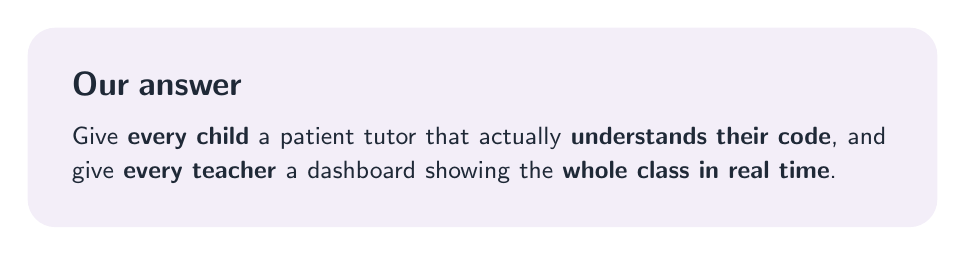
\begin{tikzpicture}
        \node[fill=scBg,rounded corners=10pt,inner sep=16pt,text width=0.86\textwidth]{%
          {\headingfont\color{scInk}\large Our answer}\\[0.6em]
          \color{scInk}\small Give \textbf{every child} a patient tutor that actually \textbf{understands their code},
          and give \textbf{every teacher} a dashboard showing the \textbf{whole class in real time}.};
      \end{tikzpicture}
  \end{columns}
\end{frame}

% ─────────────────────────── PILLARS ───────────────────────────
\begin{frame}{Three pillars}
  \vspace{1.0em}
  \begin{columns}[T,onlytextwidth]
    \column{0.31\textwidth}
      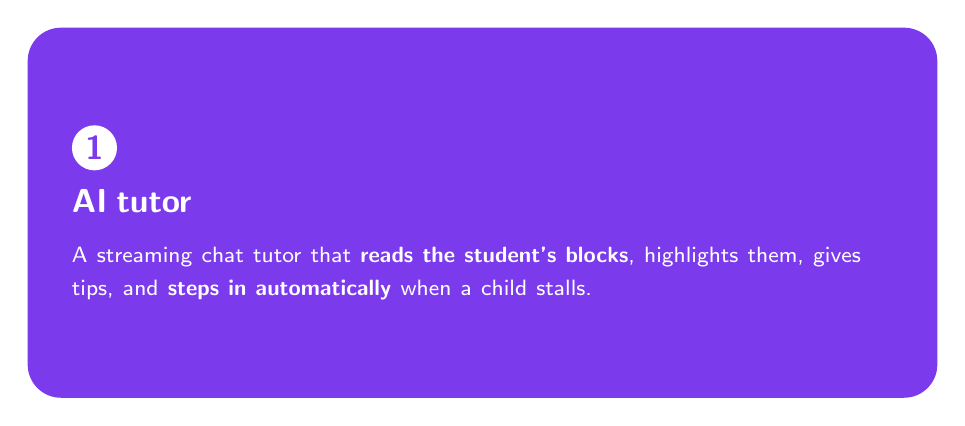
\begin{tikzpicture}
        \node[fill=scPurple,text=white,rounded corners=12pt,inner sep=16pt,text width=0.86\textwidth,minimum height=4.7cm,anchor=north]{%
          \badge{scPurple}{1}\\[0.6em]
          {\headingfont\large AI tutor}\\[0.6em]
          \footnotesize A streaming chat tutor that \textbf{reads the student's blocks}, highlights them, gives tips, and \textbf{steps in automatically} when a child stalls.};
      \end{tikzpicture}
    \column{0.31\textwidth}
      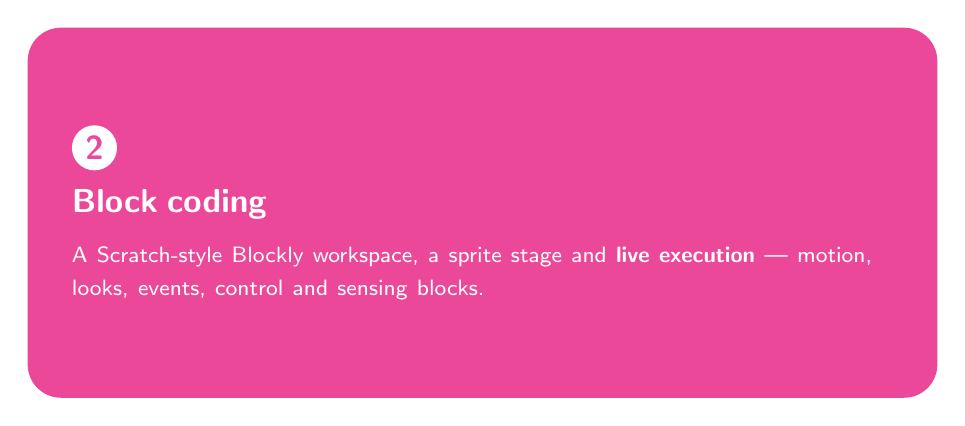
\begin{tikzpicture}
        \node[fill=scPink,text=white,rounded corners=12pt,inner sep=16pt,text width=0.86\textwidth,minimum height=4.7cm,anchor=north]{%
          \badge{scPink}{2}\\[0.6em]
          {\headingfont\large Block coding}\\[0.6em]
          \footnotesize A Scratch-style Blockly workspace, a sprite stage and \textbf{live execution} --- motion, looks, events, control and sensing blocks.};
      \end{tikzpicture}
    \column{0.31\textwidth}
      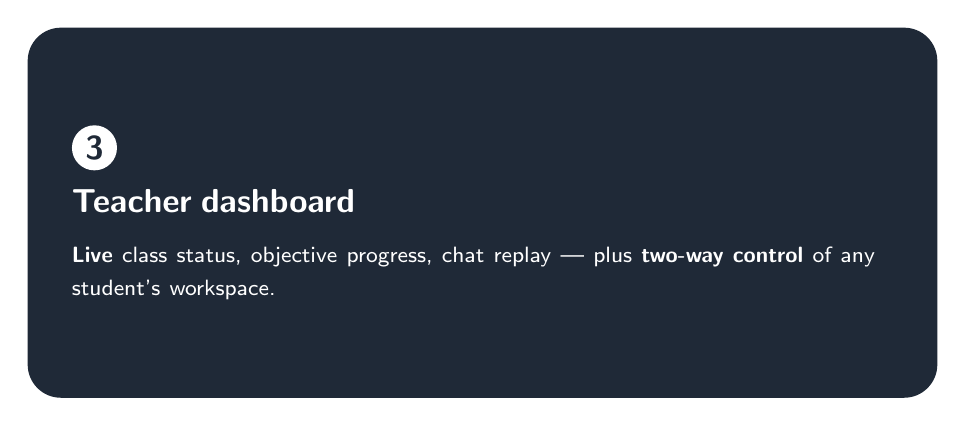
\begin{tikzpicture}
        \node[fill=scInk,text=white,rounded corners=12pt,inner sep=16pt,text width=0.86\textwidth,minimum height=4.7cm,anchor=north]{%
          \badge{scInk}{3}\\[0.6em]
          {\headingfont\large Teacher dashboard}\\[0.6em]
          \footnotesize \textbf{Live} class status, objective progress, chat replay --- plus \textbf{two-way control} of any student's workspace.};
      \end{tikzpicture}
  \end{columns}
\end{frame}

% ─────────────────────────── SECTION: HOW IT WORKS ───────────────────────────
{\setbeamertemplate{footline}{}
\begin{frame}[plain]
  \bgband
  \begin{tikzpicture}[remember picture,overlay]
    \node[text=white] at (current page.center){\headingfont\fontsize{34}{40}\selectfont How it works};
    \node[text=white!85,font=\large] at ([yshift=-1.3cm]current page.center){The moving parts, before we look at the screens};
  \end{tikzpicture}
\end{frame}}

% App flow (end to end)
\begin{frame}{End to end, in one picture}
\vspace{0.2em}
\begin{center}
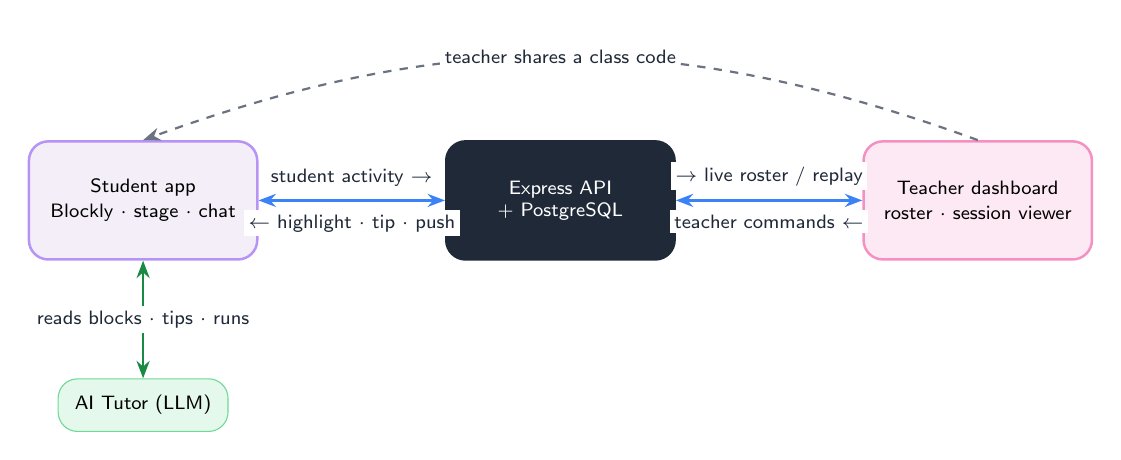
\begin{tikzpicture}[
  font=\scriptsize, >={Stealth[length=2.2mm]},
  core/.style={rounded corners=7pt,draw,line width=0.9pt,align=center,inner sep=7pt,
               minimum height=1.5cm,minimum width=2.9cm},
  app/.style={core,fill=scBg,draw=scPurple!55},
  api/.style={core,fill=scInk,text=white,draw=scInk},
  dashb/.style={core,fill=scPink!12,draw=scPink!60},
  ai/.style={rounded corners=7pt,fill=scGreen!12,draw=scGreen!65,align=center,inner sep=6pt},
  lbl/.style={font=\fontsize{7}{8.4}\selectfont,fill=white,inner sep=1.6pt,text=scInk},
]
\node[app]   (app)  at (0,0)    {Student app\\[1pt]\fontsize{7}{8}\selectfont Blockly $\cdot$ stage $\cdot$ chat};
\node[api]   (api)  at (5.3,0)  {Express API\\+ PostgreSQL};
\node[dashb] (dash) at (10.6,0) {Teacher dashboard\\[1pt]\fontsize{7}{8}\selectfont roster $\cdot$ session viewer};
\node[ai]   (ai)   at (0,-2.6) {AI Tutor (LLM)};

% AI tutor <-> app
\draw[<->,line width=1.0pt,scGreen!70!black] (ai) -- node[lbl]{reads blocks $\cdot$ tips $\cdot$ runs} (app);
% SSE both ways
\draw[<->,line width=1.2pt,scBlue] (app) -- (api);
\draw[<->,line width=1.2pt,scBlue] (api) -- (dash);
\node[lbl,above] at ($(app)!0.5!(api)+(0,0.12)$){student activity $\to$};
\node[lbl,below] at ($(app)!0.5!(api)-(0,0.12)$){$\leftarrow$ highlight $\cdot$ tip $\cdot$ push};
\node[lbl,above] at ($(api)!0.5!(dash)+(0,0.12)$){$\to$ live roster / replay};
\node[lbl,below] at ($(api)!0.5!(dash)-(0,0.12)$){teacher commands $\leftarrow$};
% join code arc (dashed) dashboard -> student
\draw[->,dashed,scGray,line width=0.8pt] (dash.north) to[bend right=20]
  node[lbl,pos=0.5]{teacher shares a class code} (app.north);
\end{tikzpicture}
\end{center}
\vspace{0.2em}
{\footnotesize\color{scGray}\hspace{0.6cm}A teacher shares a code; students join and code with the AI tutor; every action streams over
\textbf{SSE} to the dashboard --- and the teacher can stream hints and edits \textbf{back}.}
\end{frame}

% Agent <-> UI
\begin{frame}{Inside the AI tutor: agent $\Leftrightarrow$ UI}
\vspace{0.05em}
\begin{center}
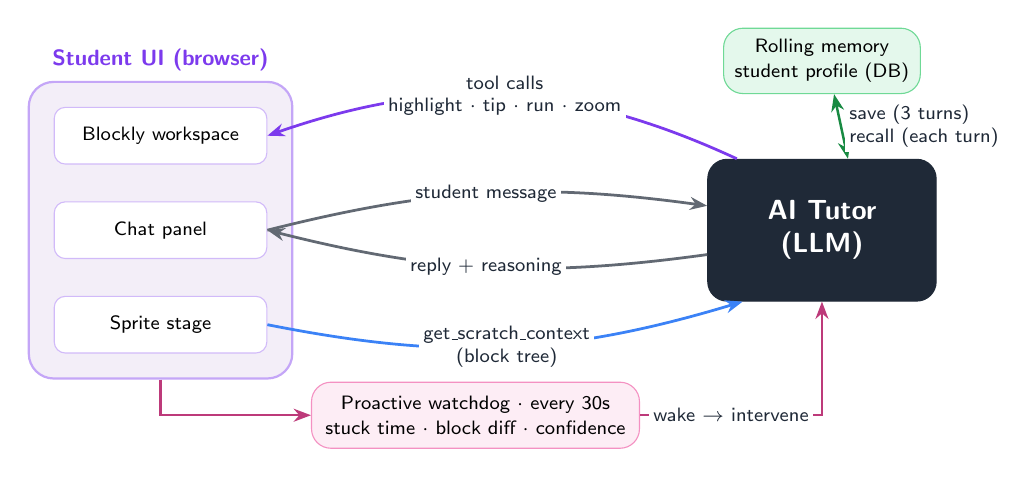
\begin{tikzpicture}[
  font=\scriptsize, >={Stealth[length=2.2mm]},
  sub/.style={rounded corners=4pt,fill=white,draw=scPurple!35,align=center,inner sep=4pt,
              minimum width=2.7cm,minimum height=0.72cm},
  llm/.style={rounded corners=7pt,fill=scInk,text=white,draw=scInk,align=center,
              minimum width=2.9cm,minimum height=1.8cm,font=\bfseries},
  mem/.style={rounded corners=7pt,fill=scGreen!12,draw=scGreen!65,align=center,inner sep=4pt},
  dog/.style={rounded corners=7pt,fill=scPink!10,draw=scPink!60,align=center,inner sep=5pt},
  lbl/.style={font=\fontsize{7}{8.2}\selectfont,fill=white,inner sep=1.6pt,text=scInk},
]
\node[sub] (ws)    at (0,1.2) {Blockly workspace};
\node[sub] (chat)  at (0,0.0)  {Chat panel};
\node[sub] (stage) at (0,-1.2){Sprite stage};
\begin{pgfonlayer}{background}
  \node[rounded corners=9pt,fill=scBg,draw=scPurple!45,line width=0.8pt,fit=(ws)(chat)(stage),inner sep=9pt](ui){};
\end{pgfonlayer}
\node[anchor=south,font=\bfseries\footnotesize,text=scPurple] at (ui.north){Student UI (browser)};

\node[llm] (llm) at (8.4,0)  {AI Tutor\\(LLM)};
\node[mem] (mem) at (8.4,2.15){Rolling memory\\[1pt]\fontsize{7}{8}\selectfont student profile (DB)};
\node[dog] (dog) at (4.0,-2.35){Proactive watchdog $\cdot$ every 30s\\[1pt]
  \fontsize{7}{8}\selectfont stuck time $\cdot$ block diff $\cdot$ confidence};

% tool calls (purple) llm -> workspace
\draw[->,line width=1.0pt,scPurple] (llm.140) to[bend right=22]
  node[lbl,pos=0.5,align=center]{tool calls\\highlight $\cdot$ tip $\cdot$ run $\cdot$ zoom} (ws.east);
% chat round trip (ink)
\draw[->,line width=1.0pt,scInk!70] (chat.east) to[bend left=11]
  node[lbl,pos=0.5]{student message} (llm.168);
\draw[->,line width=1.0pt,scInk!70] (llm.192) to[bend left=11]
  node[lbl,pos=0.5]{reply + reasoning} (chat.east);
% block context (blue) stage -> llm
\draw[->,line width=1.0pt,scBlue] (stage.east) to[bend right=14]
  node[lbl,pos=0.5,align=center]{get\_scratch\_context\\(block tree)} (llm.222);
% memory (green)
\draw[<->,line width=0.9pt,scGreen!70!black] (llm.70) --
  node[lbl,right=1pt,align=left]{save (3 turns)\\recall (each turn)} (mem.290);
% watchdog (pink)
\draw[->,line width=0.9pt,scPink!80!black] (ui.south) |- (dog.west);
\draw[->,line width=0.9pt,scPink!80!black] (dog.east) -|
  node[lbl,pos=0.25]{wake $\to$ intervene} (llm.south);
\end{tikzpicture}
\end{center}
\vspace{0.2em}
\begin{center}{\footnotesize\color{scGray}Each turn the tutor \textbf{reads the live block tree} and \textbf{acts on the UI} via tool calls; a \textbf{watchdog} wakes it when a student stalls.}\end{center}
\end{frame}

% ─────────────────────────── SECTION: STUDENT ───────────────────────────
{\setbeamertemplate{footline}{}
\begin{frame}[plain]
  \bgband
  \begin{tikzpicture}[remember picture,overlay]
    \node[text=white] at (current page.center){\headingfont\fontsize{34}{40}\selectfont The student experience};
    \node[text=white!85,font=\large] at ([yshift=-1.3cm]current page.center){From joining a class to coding with an AI by your side};
  \end{tikzpicture}
\end{frame}}

% Join
\begin{frame}{One code, and you're in}
  \begin{columns}[c]
    \column{0.38\textwidth}
      \begin{itemize}
        \item The teacher shares a \textbf{class code}
        \item Students enter the code and a name --- \textbf{no signup, no password}
        \item Identity is remembered, so they \textbf{pick up where they left off}
      \end{itemize}
    \column{0.62\textwidth}
      \shot[0.78\paperheight]{shots/01-join.png}
  \end{columns}
\end{frame}

% Hero
\begin{frame}{The AI tutor reads your blocks}
  \shot[0.80\paperheight]{shots/02-student-workspace.png}
  \shotcaption{The tutor sees the ``repeat 10'' loop, \textbf{highlights the block}, leaves an \textbf{inline tip}, and congratulates the student when the objective is met.}
\end{frame}

% Run
\begin{frame}{Hit the green flag --- the sprite comes alive}
  \begin{columns}[c]
    \column{0.62\textwidth}
      \shot[0.80\paperheight]{shots/03-student-running.png}
    \column{0.38\textwidth}
      \begin{itemize}
        \item Blocks \textbf{compile to code and run instantly}
        \item The sprite moves, talks and changes costume on the \textbf{stage}
        \item Green-flag, key, click and broadcast \textbf{events}
        \item Multiple built-in \textbf{costumes and sprites}
      \end{itemize}
  \end{columns}
\end{frame}

% ─────────────────────────── SECTION: TEACHER ───────────────────────────
{\setbeamertemplate{footline}{}
\begin{frame}[plain]
  \bgband
  \begin{tikzpicture}[remember picture,overlay]
    \node[text=white] at (current page.center){\headingfont\fontsize{34}{40}\selectfont The teacher dashboard};
    \node[text=white!85,font=\large] at ([yshift=-1.3cm]current page.center){The whole class's progress, on one screen};
  \end{tikzpicture}
\end{frame}}

% Classes
\begin{frame}{Class management}
  \begin{columns}[c]
    \column{0.38\textwidth}
      \begin{itemize}
        \item Secure login (httpOnly JWT)
        \item \textbf{Create a class} and generate a join code in one click
        \item Live \textbf{student and session counts} per class
      \end{itemize}
    \column{0.62\textwidth}
      \shot[0.6\paperheight]{shots/05-teacher-classes.png}
  \end{columns}
\end{frame}

% Roster
\begin{frame}{The class, live}
  \shot[0.64\paperheight]{shots/06-teacher-classdetail.png}
  \vspace{-0.1em}
  \begin{columns}[T,onlytextwidth]
    \column{0.33\textwidth}\footnotesize {\color{scGreen}\textbf{$\bullet$}} Who's online (active in 90s)
    \column{0.33\textwidth}\footnotesize Per-objective \textbf{completion progress}
    \column{0.33\textwidth}\footnotesize AI-intervention count \& latest blocks
  \end{columns}
\end{frame}

% Session viewer
\begin{frame}{Drill into one student}
  \shot[0.78\paperheight]{shots/07-teacher-session-blocks.png}
  \shotcaption{\textbf{Chat replay} on the left, the \textbf{live workspace} on the right; the \emph{AI memory} banner is the rolling profile the tutor builds across sessions.}
\end{frame}

% Two-way control
\begin{frame}{Two-way live control}
  \begin{columns}[c]
    \column{0.40\textwidth}
      The teacher can \textbf{step into} a student's workspace in real time:
      \begin{itemize}
        \item \textbf{Highlight} a block
        \item Leave an \textbf{inline tip} on a block
        \item \textbf{Push} an edited workspace straight to the student
      \end{itemize}
      \vspace{0.5em}
      \footnotesize\color{scGray}And inspect the JavaScript Blockly generates.
    \column{0.60\textwidth}
      \shot[0.74\paperheight]{shots/08-teacher-session-code.png}
  \end{columns}
\end{frame}

% Timeline
\begin{frame}{Activity timeline \& intervention impact}
  \begin{columns}[c]
    \column{0.60\textwidth}
      \shot[0.78\paperheight]{shots/09-teacher-session-timeline.png}
    \column{0.40\textwidth}
      \begin{itemize}
        \item \textbf{Messages, runs, stuck states, confidence and completions} in time order
        \item Every \textbf{proactive AI intervention} and its outcome
        \item Auto-computed \textbf{effectiveness} (helped / resolved)
      \end{itemize}
  \end{columns}
\end{frame}

% ─────────────────────────── TECH ───────────────────────────
\begin{frame}{Architecture}
  \vspace{0.5em}
  \begin{columns}[T]
    \column{0.5\textwidth}
      {\color{scPurple}\headingfont\large Frontend}
      \begin{itemize}\footnotesize
        \item React 19 + TypeScript + Vite
        \item Google Blockly v12 (custom Scratch blocks + JS generator)
        \item Streaming chat with reasoning display
      \end{itemize}
      \vspace{0.4em}
      {\color{scPink}\headingfont\large Backend}
      \begin{itemize}\footnotesize
        \item Express.js + cookie JWT auth
        \item PostgreSQL via Prisma ORM
      \end{itemize}
    \column{0.5\textwidth}
      {\color{scBlue}\headingfont\large Realtime}
      \begin{itemize}\footnotesize
        \item Server-Sent Events, both directions
        \item Teacher $\Leftrightarrow$ student command channel
      \end{itemize}
      \vspace{0.4em}
      {\color{scGreen!60!black}\headingfont\large AI tutor}
      \begin{itemize}\footnotesize
        \item OpenAI-compatible LLM backend
        \item Tool calls: read blocks, highlight, tip, run
        \item Background watchdog that \textbf{intervenes when stuck}
        \item Rolling student memory across sessions
      \end{itemize}
  \end{columns}
\end{frame}

% ─────────────────────────── CLOSING ───────────────────────────
{\setbeamertemplate{footline}{}
\begin{frame}[plain]
  \bgband
  \begin{tikzpicture}[remember picture,overlay]
    \node[anchor=west,text=white] at ([xshift=1.0cm]current page.west) {%
      \begin{minipage}{0.84\paperwidth}
        {\headingfont\fontsize{30}{36}\selectfont Recap}\\[0.9em]
        {\fontsize{13.5}{21}\selectfont
        $\bullet$\; Every child gets an AI tutor that \textbf{understands their blocks}\\[0.45em]
        $\bullet$\; A complete \textbf{block-coding} environment with a live stage\\[0.45em]
        $\bullet$\; Teachers get a \textbf{real-time, whole-class} dashboard with two-way control\\[0.45em]
        $\bullet$\; The AI builds a \textbf{rolling profile} of each student over time}\\[1.3em]
        {\color{white!88}\large Kids code with blocks, an AI guides them, and teachers see everything.}
      \end{minipage}};
  \end{tikzpicture}
\end{frame}}

\end{document}
